%% Template for ENG 401 reports
%% by Robin Turner
%% Adapted from the IEEE peer review template

%
% note that the "draftcls" or "draftclsnofoot", not "draft", option
% should be used if it is desired that the figures are to be displayed in
% draft mode.

\documentclass{article}
\usepackage{url} % Provides better formatting of URLs.
\usepackage[utf8]{inputenc} % Allows Spanish characters.
\usepackage[spanish]{babel}
\usepackage{amssymb}
\usepackage{booktabs} % Allows the use of \toprule, \midrule and \bottomrule in tables for horizontal lines
\usepackage{float}
\usepackage{graphicx}
\usepackage{booktabs}
\usepackage{fancyhdr}


\hyphenation{op-tical net-works semi-conduc-tor} % Corrects some bad hyphenation 



\begin{document}
%\begin{titlepage}
% paper title
% can use linebreaks \\ within to get better formatting as desired
\title{
\includegraphics[scale=0.65]{logoDefinitivo1.png} \\ \textbf{Proyecto UPBEAT} \\ \textbf{Grupo 03. Barbara Liskov}\\Propuesta técnica y económica del proyecto \vspace{0.1cm} \\}

% author names and affiliations

\author{Alejandro Ruiz Sumelzo\\
Alejandro Piedrafita Barrantes\\
Álvaro Santamaría De la Fuente\\
Fernando Navarro Zarralanga\\
José Félix Yagüe Royo\\
Víctor Pérez Sanmartín\\
Sergio Torres Castillo \vspace{0.25cm}
\\\\

\includegraphics[scale=0.5]{logoUZ.png}\\
}
\date{24 de febrero de 2020}

% make the title area
\maketitle
\newpage
\section*{Resumen ejecutivo}
En este documento se detalla la propuesta técnica y económica del proyecto \textit{UPBEAT}.

El proyecto tiene como objetivo crear un servicio de streaming de música y un cliente web que lo utilice, además de una aplicación móvil. El servidor contará con una \textit{API REST} para intercambiar datos entre el servidor y los clientes, permitiendo a estos realizar las operaciones cotidianas de una aplicación streaming de música.
\hfill\break
La descripción técnica especifica que se desarrollará el sistema sobre una capa de aplicación web basada en Angular, cumplimentado con ello una app móvil para el uso del sistema.
Esto permitirá usar servicios \textit{REST}, con \textit{Spring} como herramienta de desarrollo. Para la base de datos, se usará una PostgreeSQL. 
\hfill\break
Para todo ello, el plan de trabajo que se ha cumplimentado y acordado ha sido establecido por el cliente, reunidos periódicamente en las reuniones con el tutor del proyecto. 
\hfill\break
Se adjunta también el presupuesto total de la inversión para el proyecto \textit{UPBEAT}, con el desglose del mismo.

\newpage
\tableofcontents % si estas líneas se comentan, se eliminan los índices
%\listoffigures
%\listoftables
\addtocontents{toc}{\hfill \textbf{Página} \par}
\newpage
\pagestyle{fancy}
\lhead{\begin{picture}(0,0) \put(0,0){\includegraphics[width=40mm]{logoEina.png}} \end{picture}}
\rhead{\begin{picture}(0,0) \put(-100.7,0){
\includegraphics[width=35mm]{logoDefinitivo3.png}} \end{picture}}
\section{Objetivos del sistema}

\subsection{Análisis de requisitos preliminar}
Se exponen los siguientes requisitos funcionales de la aplicación:
\begin{table}[H]
	\begin{tabular}{p{4cm} p{10cm}}
		\hline
		\hline 
		\textbf{Requisito funcional}
		\vspace{0.5mm} & \textbf{Descripción} \\ 
		\hline
		\hline
		RF1
		& El sistema permite almacenar canciones y podcasts en formato \textit{.mp3}, \textit{.WAV} y \textit{.WMA}. \\ 
		\hline 
		RF2
		& El usuario accede al sistema mediante una aplicación móvil o una aplicación web. \\ 
		\hline
		RF3
		& El artista accede al sistema mediante una aplicación web. \\ 
		\hline
		RF4
		& El sistema permite reproducir y pausar una canción. También permite saltar a la siguiente (si la hubiera), retroceder a la anterior, y elegir un bucle de la misma o reproducir aleatoriamente varias canciones. \\ 
		\hline
		RF5
		& El sistema permite al usuario registrado subir o bajar el volumen de la canción/podcast en reproducción. \\ 
		\hline
		RF6
		& El usuario debe registrarse en el sistema o iniciar sesión para acceder a sus funcionalidades. \\ 
		\hline
		RF7
		& El usuario y el artista acceden al sistema mediante un nombre identificatorio y una contraseña. \\ 
		\hline
		RF8
		& El usuario registrado puede buscar canciones, álbumes, artistas y podcasts. \\ 
		\hline
		RF9
		& El usuario registrado puede crear playlists (agrupación de una o varias canciones) . \\ 
		\hline
		RF10
		& El usuario registrado puede añadir/eliminar de sus favoritos una canción, playlist, álbum o podcast . \\ 
		\hline
		RF11
		& El usuario registrado puede ordenar por fecha de lanzamiento, nombre y por artista las canciones añadidas a una playlist. \\ 
		\hline
		RF12
		&  El usuario registrado puede seguir a otros usuarios dentro del sistema.\\
		\hline
		RF13
		&  El usuario registrado puede filtrar la búsqueda de una determinada canción por género y época.\\
		\hline
		RF14
		&  El sistema permite sincronizar varios dispositivos, de tal manera que si reproduces la misma canción con el mismo usuario registrado en distintos dispositivos, solo puedas hacerlo en uno de ellos.\\
		\hline
		RF15
		&  El sistema permitirá tener \textit{banner} de anuncios en la aplicación web.\\
		\hline
		RF16
		& El sistema permite al usuario registrado manejar un equalizador del sonido. \\ 
		\hline
		RF17
		& El artista tiene todas las funcionalidades del usuario registrado, además de poder subir canciones y podcast. \\ 
		\hline
		RF18
		& El artista puede elegir la fecha y hora de una publicación, o subirla inmediatamente. \\ 
		\hline
	\end{tabular}
\end{table}
\break
Se exponen los siguientes requisitos no funcionales de la aplicación:

\begin{table}[H]
	\begin{tabular}{p{4cm} p{10cm}}
		\hline
		\hline 
		\textbf{Requisito no funcional} & \textbf{Descripción} \\ 
		\hline
		\hline
		RNF1 
		&  El sistema permitirá ser utilizar un diseño modular, un lenguaje fácil de entender, usar y mantener.\\ 
		\hline
		RNF2
		&  La seguridad será fundamental a la hora de garantizar la confidencialidad y autentificación de las canciones, así como para cumplir determinados aspectos de la LOPD y los derechos de los cantautores.\\ 
		\hline
		RNF3
		&  El cliente tendrá el desarrollo móvil en formato Android e iOS.\\ 
		\hline
	\end{tabular}
\end{table}
\newpage

\section{Descripción técnica}

\subsection{Aspectos técnicos para el usuario}
El usuario solamente necesitará de un navegador web para conseguir conectarse al proyecto \textit{UPBEAT}.
Este proyecto será compatible con el navegador \textit{Google Chrome}.\vspace{0.5cm}
\hfill\break
\begin{figure}[H]
	\centering{

\includegraphics[scale=0.38]{navegadorWeb.png}}
\end{figure}

\subsection{Aspectos técnicos para el cliente}
El proyecto será entregado en un servidor web de hosting, el cual implementará todos los servicios necesarios para que funcione correctamente. Se le proporcionará un usuario y contraseña para acceder al mismo y hacerse cargo una vez se desarrolle y entregue el proyecto.
\hfill \break
También se le proporcionará al cliente los archivos de ambas aplicaciones desarrolladas para la tecnología móvil.
\begin{figure}[H]
	\centering{
		
\includegraphics[scale=0.35]{android-apple.png}}
\end{figure}

\newpage
\subsection{Descripción técnica preliminar}
Para la realización del proyecto, el sistema usará la siguiente estructura: \vspace{0.15cm}

\begin{figure}[H]
	\centering{
	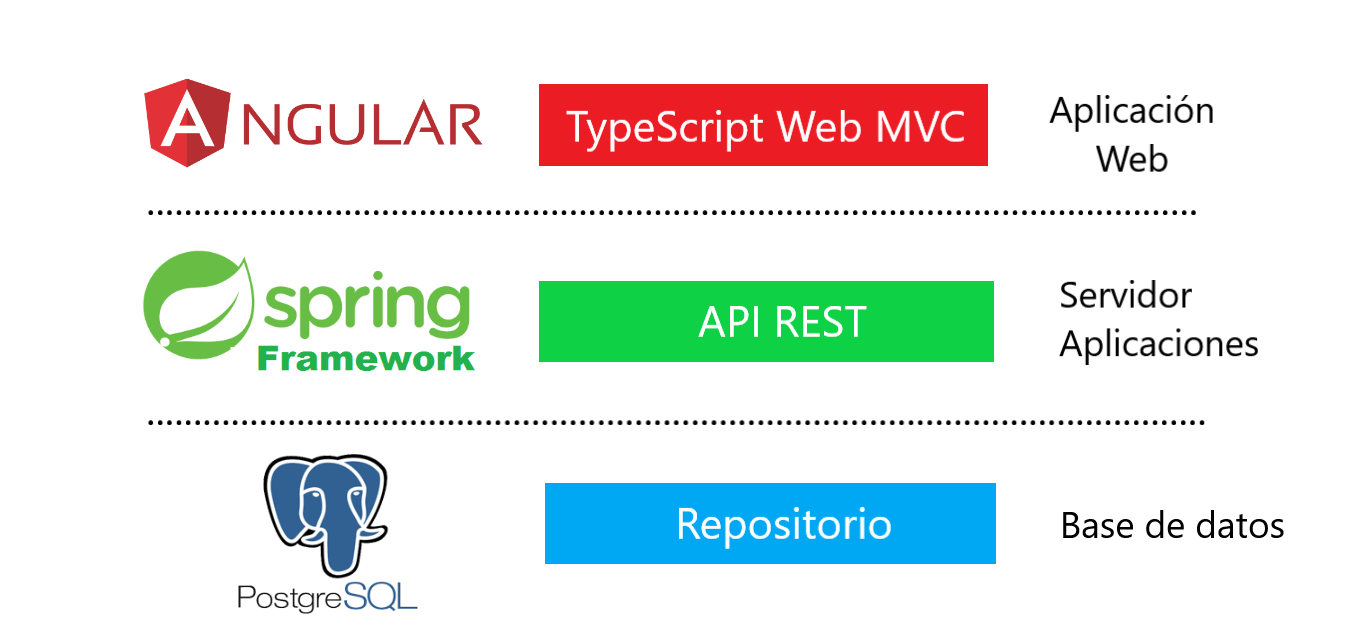
\includegraphics[scale=0.35]{EstructuraProyecto.png}}
\end{figure}
\vspace{0.15cm}

El desarrollo del cliente web se centrará en \textit{Angular} principalmente, el cual se conectará al servidor de aplicaciones que proporcionará \textit{Spring Boot}. Este último gestionará las consultas y conexiones con la base de datos, desarrollada e implementada en \textit{PostgreSQL}.
Para el desarrollo de la aplicación móvil se usará \textit{Flutter}:
\begin{figure}[H]
	\centering{
		
\includegraphics[scale=0.55]{flutter.png}}
\end{figure}
\newpage

\section{Plan de trabajo}
\begin{itemize}
	\item ¿Qué se va a entregar?
	\begin{itemize}
		\item \textbf{Propuesta técnica y económica}: requisitos, prototipos de diseño, presupuesto y costes.
		\item \textbf{Prototipo funcional del sistema}, el cual va a ir evolucionando a medida que avanza el proyecto, con el objetivo de obtener feedback del cliente.
		\item \textbf{Manual de usuario}.
	\end{itemize}
\end{itemize}

\begin{itemize}
	\item ¿Cuándo se va a entregar?
	\begin{itemize}
		\item \textbf{Entrega 1: plan de trabajo. 24/02/2020}
		Propuesta técnica y económica.
		\item \textbf{Entrega 2: diseño y arquitectura. 12/03/2020}
		Prototipo de alto nivel en el que el cliente puede ver como se comporta la aplicación, pero aún no es funcional.
		\item \textbf{Entrega 3: implementación. 18/04/2020}
		Prototipo de alto nivel funcional con el que el cliente puede comprobar el correcto funcionamiento de la aplicación.
		\item \textbf{Entrega 4: entrega final. 8/05/2020}
		Prototipo final junto con el manual de usuario.
	\end{itemize}
\end{itemize}

\newpage

\section{Equipo técnico encargado del proyecto}
La empresa \textit{UPBEAT SA}, dedicada al desarrollo de proyectos de software por demanda, está compuesta por 7 estudiantes de la titulación de Ingeniería Informática en la Universidad de Zaragoza, los cuales cursan las ramas de sistemas de la información y administración de sistemas.
\hfill \break
Previamente, se han desarrollado proyectos relacionados con el trabajo a desempeñar, en los cuales se desarrolló e implementó una aplicación web de recomendación de automóviles de bajo consumo. Unido a esto, también se creó todo la gestión de usuarios del sistema.
\hfill \break
La empresa también cuenta experiencia en varias tecnologías punteras en el mercado, como Docker o Angular, este último trabajado en proyectos de integración de logística empresarial.
La empresa en la que se ha trabajado con proyectos similares ha sido Carreras Grupo Logístico.
\hfill \break
Varios de los integrantes de la compañía poseen años de experiencia laboral que permiten asegurar el éxito del proyecto expuesto en este documento.


\newpage

\section{Presupuesto}
\textit{D. ALEJANDRO RUIZ SUMELZO}, domiciliado para estos efectos en Zaragoza, provincia de Zaragoza, calle \textit{Camino de Juslibol N.º 36}, y DNI \textit{25203767E} en nombre y representación de \textit{UPBEAT S.A.} con C.I.F. \textit{123456} y domicilio fiscal en Zaragoza, calle \textit{María de Luna}, edificio \textit{Ada Byron}, enterado del anuncio publicado en el Moodle de la Universidad de Zaragoza, a día 13 de febrero de 2020 y de las condiciones y requisitos que se exigen para la adjudicación de los servicios de la \textbf{REALIZACIÓN DE UNA APLICACIÓN DE REPRODUCCIÓN DE MÚSICA}, provincia de ZARAGOZA, se compromete a tomar a su cargo la ejecución de los mismos, con estricta sujeción a los requisitos y condiciones expresados, por las cantidades que se enumeran en concepto de precio, indicándose igualmente el IVA a soportar por la Administración, en cada caso, según las soluciones siguientes:

\begin{figure}[H]
	\centering{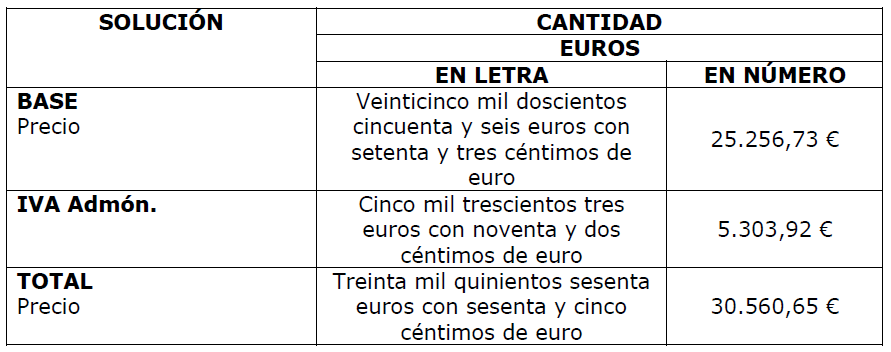
\includegraphics[scale=0.65]{PropuestaTabla.png}}
\end{figure}

El licitador hace constar que el precio o precios del contrato ofertado incluye el importe de las tasas que sean de aplicación, con conformidad con lo señalado en el Pliego de Cláusulas Administrativas Particulares que rige este contrato. 
\newpage
\section*{Anexo I. Estimación de costes}
\begin{figure}[H]
	\hspace*{-3.5cm}
	\centering{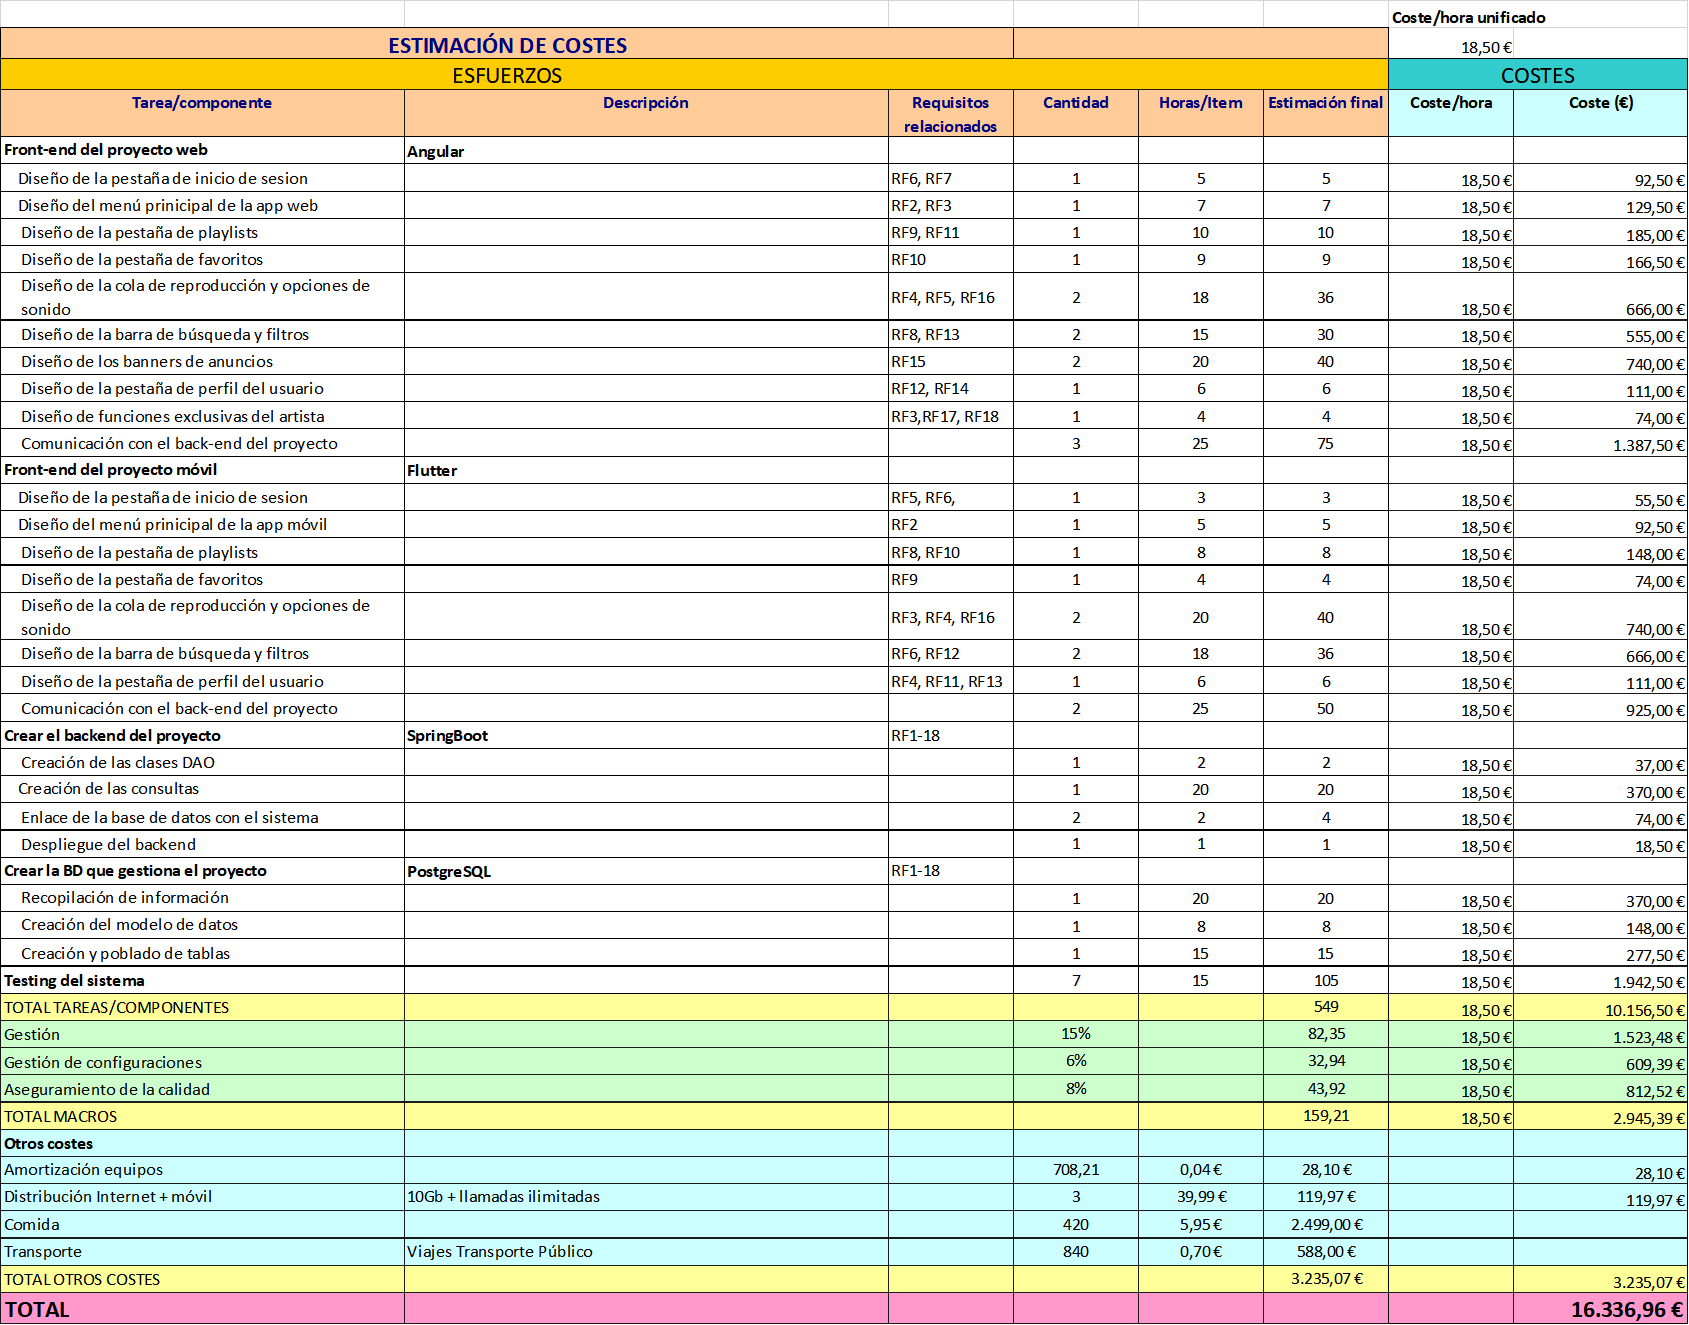
\includegraphics[scale=0.7]{EstimacionCoste.png}}
\end{figure}

\end{document}


